% !TeX spellcheck = en_US
\documentclass[12pt]{article}

\usepackage{times,fullpage,xspace,fancyhdr,url,color}
\usepackage[pdftex]{graphicx}
\usepackage[pdftex,
            colorlinks=true,
            urlcolor=black,
            linkcolor=black,
            citecolor=black,
            bookmarksopen=false,
            bookmarksnumbered=true,
            pdfstartview=FitH]{hyperref}

\pdfcompresslevel=9
\newcommand{\leaguename}{RoboCup Standard Platform League (NAO) }
\hypersetup{
 pdftitle={\leaguename Technical Challenges},
 pdfauthor={Technical Committee SPL},
}
\usepackage{microtype}
\usepackage[utf8]{inputenc}
\usepackage{amsmath}
\usepackage{xargs}
\usepackage[colorinlistoftodos,prependcaption,textsize=tiny]{todonotes}
\usepackage{siunitx}
\usepackage[capitalize,noabbrev]{cleveref}
\usepackage[official]{eurosym}
\usepackage[useregional]{datetime2}
\usepackage{subcaption}
\usepackage{enumitem}
\usepackage{xcolor}
\DTMlangsetup[en-GB]{ord=raise,monthyearsep={,\space}}

\newcommandx{\unsure}[2][1=]{\todo[linecolor=red,backgroundcolor=red!25,bordercolor=red,#1]{#2}}
\newcommandx{\change}[2][1=]{\todo[linecolor=blue,backgroundcolor=blue!25,bordercolor=blue,#1]{#2}}
\newcommandx{\info}[2][1=]{\todo[linecolor=green,backgroundcolor=green!25,bordercolor=green,#1]{#2}}
\newcommandx{\improvement}[2][1=]{\todo[linecolor=Plum,backgroundcolor=Plum!25,bordercolor=Plum,#1]{#2}}

% comment 'disable' in to disable all the todo notes :)
\usepackage
[
%disable
]{todonotes}

\usepackage[theorems]{tcolorbox}
\newtcbtheorem[number within=section]{hintbox}{}%
{colback=red!10,colframe=red!45!black,fonttitle=\bfseries}{th}

% !TeX root = ../SPL-Rules.tex
% !TeX spellcheck = en_US
\newcommand{\TotalWidth}{7.4}
\newcommand{\TotalLength}{10.4}
\newcommand{\GoalScoredDelay}{15}
\newcommand{\KickOffAutoTime}{45}
\newcommand{\KickOffBallFreeTime}{10}
\newcommand{\FreeKickTime}{30}
\newcommand{\FreeKickRadius}{0.75}
\newcommand{\VisualSignalTime}{2}
\newcommand{\ReadyDelayTimeChampion}{45}
\newcommand{\ReadyDelayTimeChallenge}{40}
\newcommand{\PlayingDelayTime}{15}
\newcommand{\PenaltyKickTime}{30}
\newcommand{\PenaltyKickSetupTime}{30}
\newcommand{\PenaltyShootoutKickTime}{30}
\newcommand{\StandardPenaltyTime}{45}
\newcommand{\StandardPenaltyIncrease}{10}
\newcommand{\NovelContributionTime}{3 years\xspace}
\newcommand{\GameStuckTime}{30}
\newcommand{\TeamMessageSize}{128}
\newcommand{\TeamMessageLimit}{1200} % Limit of number of packets available to one team during a game with two halves of 10 minutes.
\newcommand{\TeamMessageLimitMinute}{60} % Limit for the average number of packets available to one team during a minute of gameplay.
\newcommand{\MaxJerseyNumber}{20} % the highest allowed jersey number to wear by robot players

% !TeX root = ../SPL-Rules.tex
% !TeX spellcheck = en_US
\newcommand{\LastRCYear}{2022\xspace}
\newcommand{\RCYear}{2023\xspace}
\newcommand{\JerseyApproveSubmissionDate}{2023-05-01}
\newcommand{\CodeReleaseAnnouncementDate}{2023-10-15}


\sloppy
\newcommand{\ie}{\mbox{i.\,e.}\xspace}
\newcommand{\eg}{\mbox{e.\,g.}\xspace}
%\newcommand{\cf}{\mbox{cf.}\xspace}
\newcommand{\cf}{see\xspace}
% \newcommand{\comment}[1]{\marginpar{\pdfannot width 4in height .5in depth 8pt {/Subtype /Text /Contents (#1)}}}
\newcommand{\inparagraph}[1]{\paragraph{#1\hspace{-1em} }}


% some colors
\definecolor{orange}{rgb}{1,0.5,0}
\definecolor{red}{rgb}{1,0,0}
\definecolor{green}{rgb}{0,1,0}


\title{\leaguename\\Technical Challenges}
\author{RoboCup Technical Committee}
\date{(DRAFT \RCYear technical challenges, as of \today)}

\setlength{\parindent}{0pt}
\setlength{\parskip}{12pt plus 6pt minus 3 pt}
\setcounter{tocdepth}{1}
\widowpenalty=10000
\clubpenalty=10000

\pagestyle{fancy}
\lhead{}
\chead{}
\rhead{}
\lfoot{}
\cfoot{}
\rfoot{}

\renewcommand{\headrulewidth}{0.4pt}
\renewcommand{\footrulewidth}{0.4pt}

% needed to align an image and text correctly side by side
\newcommand{\imagebox}[1]{\raisebox{2ex}{\raisebox{-\height}{#1}}}

\begin{document}

\maketitle

\vfill
\tableofcontents
\setcounter{tocdepth}{3}
\thispagestyle{fancy}
\clearpage
\cfoot{\thepage}
\setcounter{page}{1}

\section{Introduction}
At RoboCup \RCYear, the Standard Platform League will hold three technical challenges, which are described in this document.
RoboCup \RCYear awards a trophy for winning the overall ranking of the three challenges and option for prequalification if a team is not prequalified by the main competition.

Technical challenges are used in SPL to develop technical capabilities which will be used in upcoming RoboCups in the main competition. The purpose is to give teams time to develop solutions and exchange ideas before they will be introduced into the main competition. Challenges are designed to move the league in a direction of further improvement  of soccer skills and towards the overall goal of 2050. Each team in strongly encouraged to participate in this challenges to contribute to the league's advancement. 

\subsection{Code publication}
It is expected that every team participating in one challenge publishes the corresponding code used in that competition according to \todo{Section in rules book}.

\subsection{Scoring}
The scores earned in each challenge will vary in magnitude. Hence, they must be scaled before calculating the overall technical challenge rankings. Teams who do not participate in a challenge will receive 0 points for that challenge. The team with the highest total score for a challenge will get 25 points for that challenge, while the team with the lowest total score for a challenge will get 5 points for that challenge. A linear equation will then be fit to these two points, and each other participating team in that challenge will gain points for that challenge based on this equation.

Questions or comments on the technical challenge rules should be mailed to \url{rc-spl-tc@lists.robocup.org}.


% !TeX root = ../SPL-Challenges.tex
% !TeX spellcheck = en_US
\section{Ingame Visual Referee Challenge}

\subsection{Challenge Goal}

In the current SPL rules, the only time that a robot is required to listen directly to the human referees is for the kick-off and goal whistle. Otherwise, all human referee decisions are communicated to the robots via electronic GameController messages. In moving towards the 2050 RoboCup goal, robots will need to directly interpret referee calls and signals (such as whistles, spoken calls and hand signals), rather than receive information from an external electronic source.
Building on the Visual Referee Challenge from 2022, this year's Ingame Visual Referee Challenge asks the robots to detect visual referee signs during a regular match when a whistle has been blown. The normal game play is not influenced by this challenge.

This technical challenge tests a robot's ability to identify three categories of hand signals during a match:
\begin{enumerate}
    \item Static hand signals with one hand.
    \item Static hand signals with two hands.
    \item Dynamic (motion) hand signals with one or two hands.
\end{enumerate}

The intent of this challenge is to choose a \emph{subset} of potential referee calls in SPL matches and test ability of a team to recognize different types of hand signals in preparation for adoption in RoboCup matches.

\subsection{Challenge setup}

As this is ingame challenge, the challenge is executed during all preliminary matches of the main competition. All usual rules apply and teams are free to participate or not.

During \textit{Set} and anytime during \textit{Playing} when the head referee whistles (Kick-off, goal, half ends), the challenged team (can be both teams) have to look to the T-junction opposite to the GameController operator. At the T-junction of the center field line a challenge assistant will show within \qty{5}{\second} after the whistle a random hand-signal and direction according to the list below for \qty{10}{\second}. The hand-signals and directions are randomly chosen but within the first four whistles there have to be hand-signals from all three classes. The same hand-signal may be chosen twice (with different directions). The challenge assistant is wearing red gloves to distinguish him from the other referees. In case the head referee has to stand on the T-junction, he will stand close to the challenge assistant and do his referee job from that close by position.

The challenge assistant must wear referee cloth and red gloves. The purpose of this clothing is to clearly distinguish the challenge assistant and its hands from the other referees and from the background people. 

The description of this challenge and hand-signals are described based on the viewpoint of the challenge assistant. In these descriptions from the perspective of the head referee the ``red team'' is defined as playing from left-to-right, and the ``blue team'' as playing from right-to-left. The use of colors for identifying teams is used to give equivalence to the head referee calls during the match \cf~\cref{fig:visual_referee_inital_positions}. Blue and red have to be replaced by the actual colors of that particular game.

The challenged team represented by the robot with the lowest number reports its evaluation of the particular hand-signal and direction using very loud sound output, repeating the result four times and sends a message with the decision over Wifi. \textbf{Details about this will come.} Only Messages with audio output and message sent within \qty{15}{second} after the signalling started will be accepted.

The challenge assistant has to decide before the match starts a suitable number of hand-signal and direction pairs and note them down. An assistant supports the challenge assistant by showing the signal and direction, taking the timing and is also listing to the answer of the robot.

\subsection{Available Hand-Signals}

Each hand-signal for the challenge is \textbf{described from the perspective of the head referee} and \textbf{pictured from the perspective of the robots}. Note that for the purpose of clarity, these do not necessarily correspond to human soccer hand-signals.

\begin{figure*}[ht!]
    \centering
    \begin{subfigure}{.33\textwidth}
        \centering
        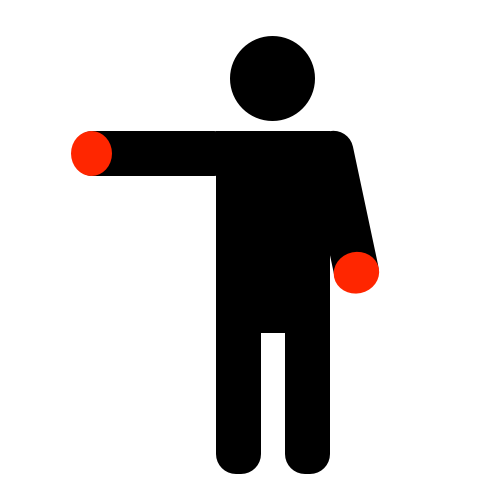
\includegraphics[height=120px]{figs/technical_challenges/kick-in.png}
        \caption{\color{blue}Kick-in \textlangle{}blue\textrangle{} Team}
    \end{subfigure}
    \begin{subfigure}{.33\textwidth}
        \centering
        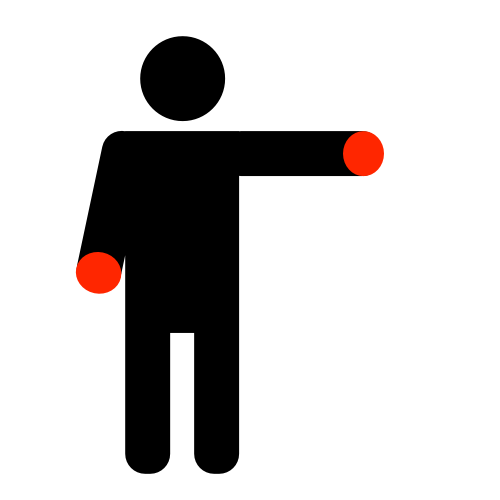
\includegraphics[height=120px]{figs/technical_challenges/kick-in-flipped.png}
        \caption{\color{red}Kick-in \textlangle{}red\textrangle{} Team}
    \end{subfigure}
    \caption{\textbf{Kick-in \textlangle{}color\textrangle{} Team.} One-handed signal. One arm, extended horizontally in the direction of the half of the field corresponding to the team that receives the Kick-in Free Kick. That is, right arm extended for the ``Blue team'', and left arm extended for the ``Red team''. The non-signal hand is flat and motionless by the side of the body.}
\end{figure*}
    
\begin{figure}[ht!]
    \centering
    \begin{subfigure}{.33\textwidth}
        \centering
        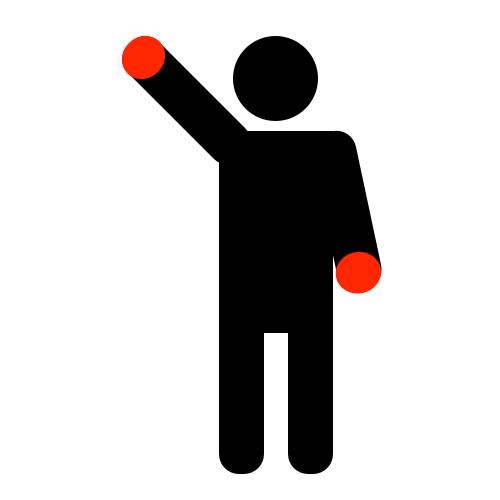
\includegraphics[height=120px]{figs/technical_challenges/goal-kick.png}
        \caption{\color{blue}Goal Kick \textlangle{}blue\textrangle{} Team}
    \end{subfigure}
    \begin{subfigure}{.33\textwidth}
        \centering
        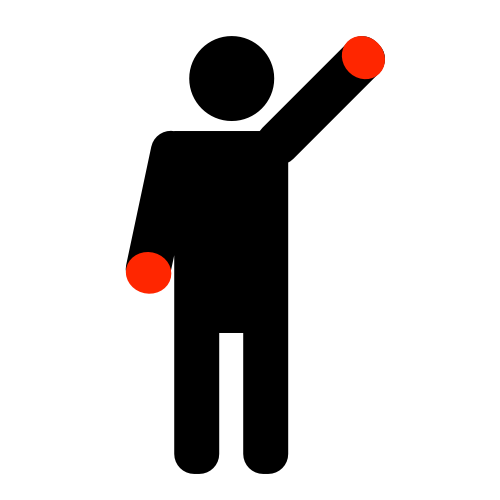
\includegraphics[height=120px]{figs/technical_challenges/goal-kick-flipped.png}
        \caption{\color{red}Goal Kick \textlangle{}red\textrangle{} Team}
    \end{subfigure}
    \caption{\textbf{Goal Kick \textlangle{}color\textrangle{} Team.} One-handed signal. One arm, extended 45-degree \emph{up} in the direction of the end of the field where the goal kick will occur. That is, right arm extended for the ``Blue team'', and left arm extended for the ``Red team''. The non-signal hand is flat and motionless by the side of the body.}
\end{figure}

\begin{figure}[ht!]
    \centering
    \begin{subfigure}{.33\textwidth}
        \centering
        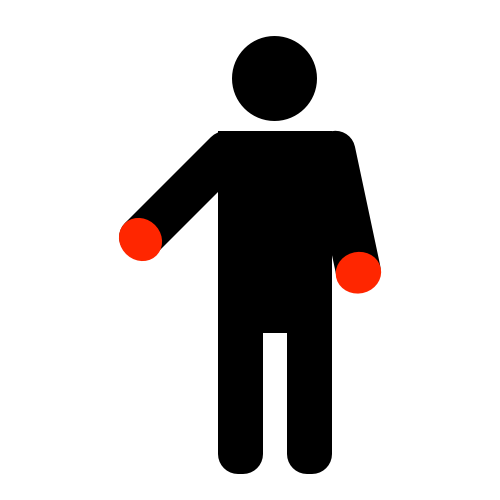
\includegraphics[height=120px]{figs/technical_challenges/corner-kick.png}
        \caption{{\color{blue}Corner Kick \textlangle{}blue\textrangle{} Team}\\ (on the half of the {\color{red} red} team)}
    \end{subfigure}
    \begin{subfigure}{.33\textwidth}
        \centering
        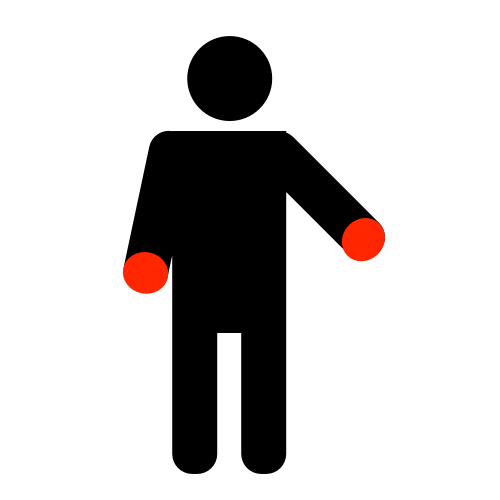
\includegraphics[height=120px]{figs/technical_challenges/corner-kick-flipped.png}
        \caption{{\color{red}Corner Kick \textlangle{}red\textrangle{} Team} (on the half of the {\color{blue} blue} team)}
    \end{subfigure}
    \caption{\textbf{Corner Kick \textlangle{}color\textrangle{} Team.} One-handed signal. One arm, extended 45-degree \emph{down} in the direction of the team executing the corner kick. That is, right arm extended for the ``Blue team'' executing the corner kick on the ``Red team's'' side, and left arm extended for the ``Red team'' executing the corner kick on the ``Blue team's'' side. The non-signal hand is flat and motionless by the side of the body.}
\end{figure}
    
\begin{figure}[ht!]
    \centering
    \begin{subfigure}{.33\textwidth}
        \centering
        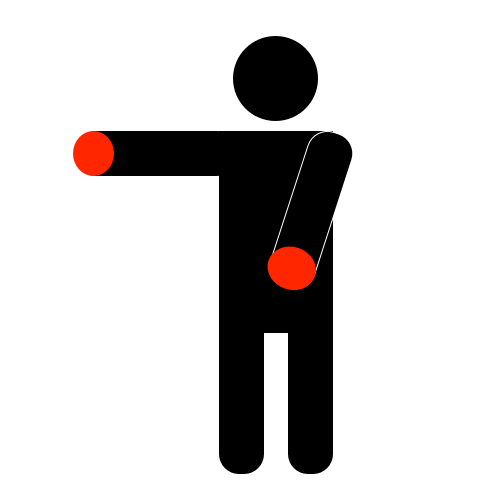
\includegraphics[height=120px]{figs/technical_challenges/goal.png}
        \caption{\color{blue}Goal \textlangle{}blue\textrangle{} Team}
    \end{subfigure}
    \begin{subfigure}{.33\textwidth}
        \centering
        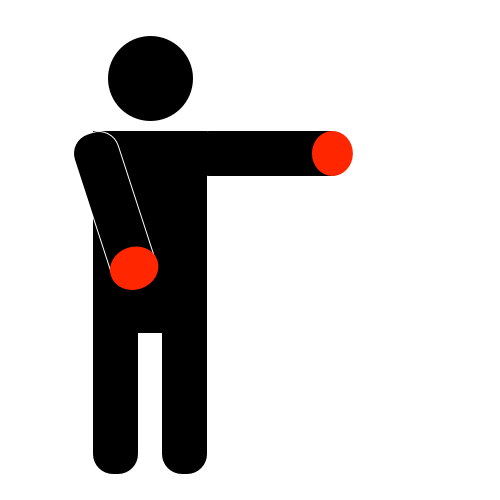
\includegraphics[height=120px]{figs/technical_challenges/goal-flipped.png}
        \caption{\color{red}Goal \textlangle{}red\textrangle{} Team}
    \end{subfigure}
    \caption{\textbf{Goal \textlangle{}color\textrangle{} Team.} Two-handed signal. One arm, extended pointing at the center circle. Other arm, extended horizontally in the direction of the half of the field corresponding to the team that scored the goal. That is, right arm extended for the ``Blue team'', and left arm extended for the ``Red team''.}
\end{figure}

\begin{figure}[ht!]
    \centering
    \begin{subfigure}{.33\textwidth}
        \centering
        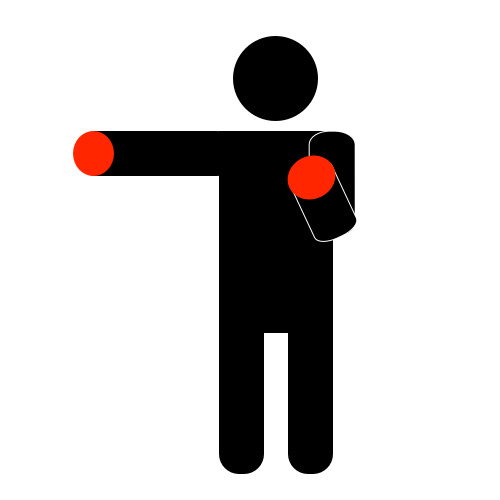
\includegraphics[height=120px]{figs/technical_challenges/pushing.png}
        \caption{{\color{blue}Pushing Free-kick \textlangle{}blue\textrangle{} Team}\\ because a {\color{red}red} robot has pushed.}
    \end{subfigure}
    \begin{subfigure}{.33\textwidth}
        \centering
        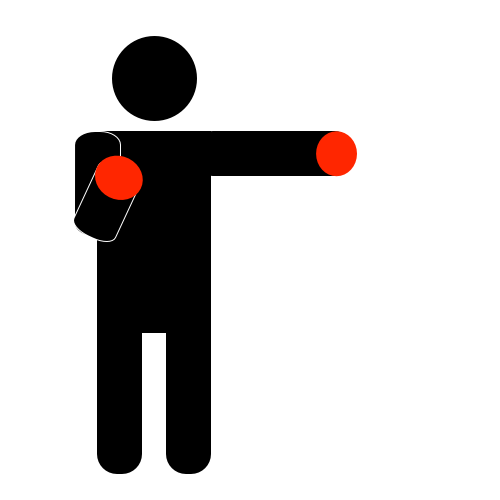
\includegraphics[height=120px]{figs/technical_challenges/pushing-flipped.png}
        \caption{{\color{red}Pushing Free-kick \textlangle{}red\textrangle{} Team}\\ because a {\color{blue}blue} robot has pushed.}
    \end{subfigure}
    \caption{\textbf{Pushing Free-kick \textlangle{}color\textrangle{} Team.} Two-handed signal. One arm, vertical with bent elbow and palm facing in the direction of the extended arm. Other arm, extended horizontally in the direction of the half of the field corresponding to the team that is \emph{executing} the Free-kick. That is, left arm extended for the ``Red team'', and right arm extended for the ``Blue team''.}
\end{figure}

\begin{figure}[ht!]
    \centering
    \begin{subfigure}{.33\textwidth}
        \centering
        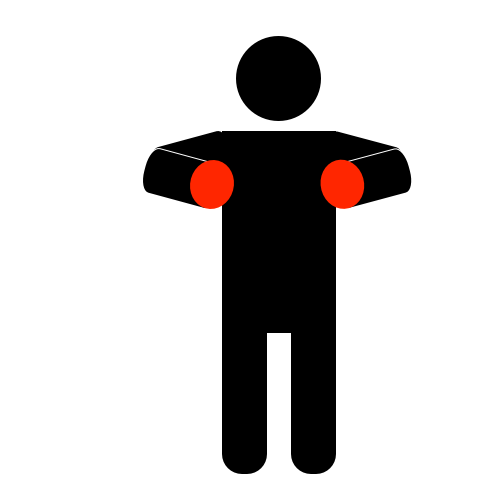
\includegraphics[height=120px]{figs/technical_challenges/full-time-start.png}
        % \caption{Inner start point of the dynamic movement}
    \end{subfigure}
    \begin{subfigure}{.33\textwidth}
        \centering
        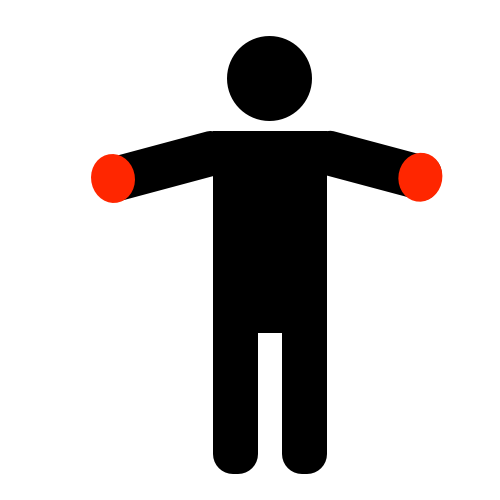
\includegraphics[height=120px]{figs/technical_challenges/full-time-end.png}
        % \caption{Outer start point of the dynamic movement}
    \end{subfigure}
    \caption{\textbf{Full-Time.} Dynamic two-handed signal. Both arms slowly move symmetrically inward and outwards on a horizontal plane, bending at the elbows. Note, for the purpose of this challenge, the whistle associated with this signal should be a \textit{single} blow, unlike in normal SPL games.}
\end{figure}

\clearpage
\subsection{Challenge evaluation}

A team scores 1 point for every hand-signal that is correctly identified. A team scores an additional 1 point for correctly identifying the team corresponding to the signal (where appropriate: For a correct recognized \textit{Full-Time} signal without announcing a team, the team gets also 1 point for the team color). A team looses 1 point for incorrectly identifying a hand-signal (note a team may have a negative final score). The total time for the robot to identify each hand-signal is summed (If a robot fails to identify a hand-signal the time for the hand-signal is \qty{15}{\second}. If a robot incorrectly identifies a hand-signal, the time is how long the robot took to provide the incorrect identification).

TODO: How to handle no goal, many goal, time out. remove best/worst, mean

Teams are ranked by their total points. In the event of tie-breaks, the team with the fastest total time to identify all hand-signals is ranked higher. The team with the highest total points, and lowest total time (for tie-breaks), wins the challenge.

% !TeX root = ../SPL-Challenges.tex
% !TeX spellcheck = en_US
\section{Dynamic Ball Handling Challenge}

This challenge is a follow-up to the Dynamic Ball Handling Challenge of RoboCup 2022 and for this new edition a few small things were changed, but especially the scoring was adjusted. The purpose of this challenge is to enhance skills in ball passing and handling, and in robot's movement estimation.  

\subsection{Challenge Goal}

Score a goal as the attacking team after two or more passes without letting the defending players touch the ball. To allow for fast attacks, each player should pass the ball to the next target without them having to walk back or turn around.

\subsection{Challenge Setup}

This challenge is executed on a standard SPL field with GameController and consists of three individual runs with time in between (the exact time is subject to the given scheduling) in which changes/adjustments to the code are allowed. Three attacking robots, provided by the challenged team, and three defending robots, operating a provided common image (see \cref{sec:Challenge_image}) from another team, are competing. For each run a new defending image will be randomly selected (if more than one image exists), so that all teams have to compete against the same image.

The defending robots have to be flashed and calibrated with the selected image for each run. Teams have to practice setting up defending robots.
It is preferable that all teams in a run play against the same robots with the same defender image. However, this is only possible if one team per round agrees to provide these robots in addition. In this case, it should be ensured that the common defenders are not actively used for more than \qty{10}{\minute} at a time, otherwise a forced break of \qty{10}{\minute} (like a half-time) must be introduced. This will be decided by the referee of this challenge.
Otherwise each team will be teamed with another team for a run. Following from this, each run is divided into two phases executed after each other. For the first phase of a run the first mentioned team brings their three attacking robots and the other team provides the defending team. During the second phase teams switch their robots respectively. 

All participating teams have to have their robots ready \qty{10}{\minute} before each challenge run starts. Attacking robots are not allowed to be modified afterwards for this run (except a robot breaks, but even than the code should remain the same except for some necessary parameters).

The robots are placed by the referees facing the opponent's half and they should allow a bit of randomness into the position same for all teams in this run.
\begin{description}
	\item[Attacker:] \textit{1st:} goal area front line; \textit{2nd:} near to center line left of center circle, but at least \qty{10}{\cm} in its own half; \textit{3rd:} next to center line right of center circle, but at least \qty{10}{\cm} in its own half.
	\item[Defender:] \textit{1st:} goalkeeper on the ground line between the two goal posts; \textit{2nd:} front line penalty area; \textit{3rd:} within center circle, but at least \qty{10}{\cm} in its own half; 
	\item[Ball:] On penalty spot of the attacking team's side
\end{description}

\begin{figure}[hb!]
	\begin{center}
		\leavevmode
		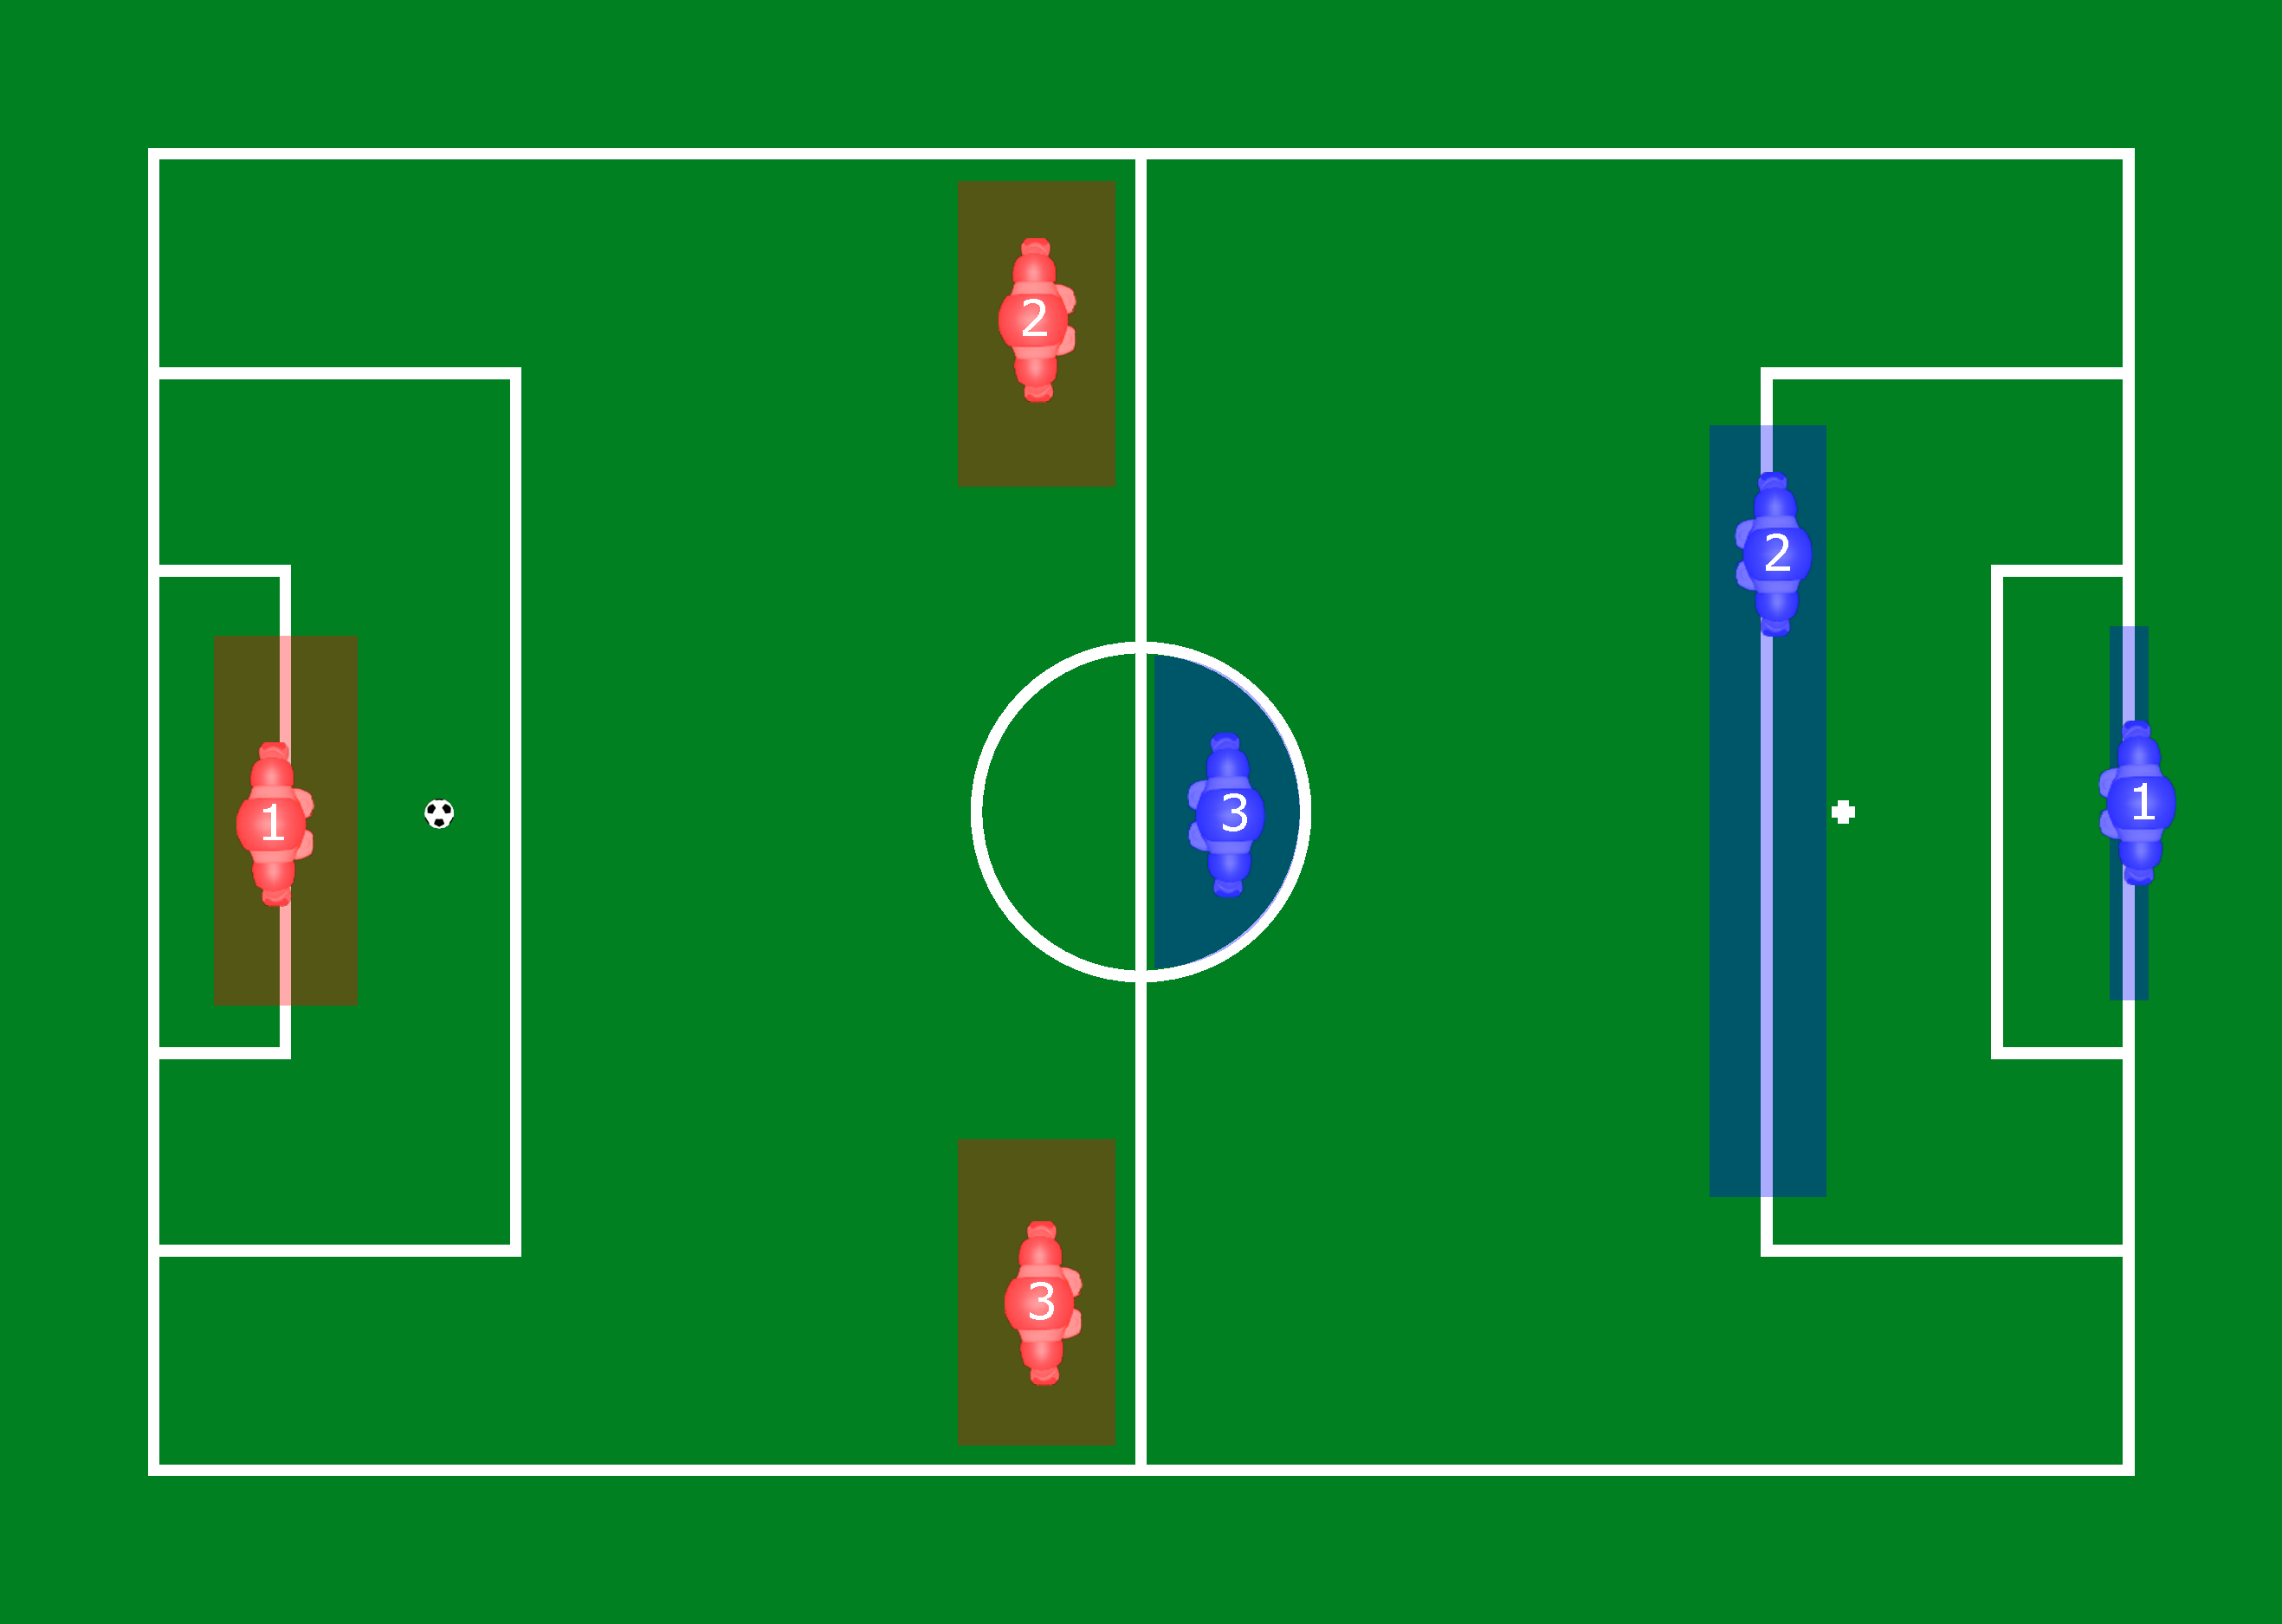
\includegraphics[width=1\columnwidth]{figs/dbhc_initial.pdf}
		\caption{Possible positions of the {\color{red}attacking (red)} and {\color{blue}defending (blue)} robots at the beginning of the challenge. All robots are facing their opponent's half and the possible randomized area is highlighted under the robots.}
		\label{fig:ball_handling_inital_positions}
	\end{center}
\end{figure}

\subsection{GameController}
All robots have to communicate with the GameController. There is a special mode in the GameController for this challenge. 

\subsection{Challenge Execution}

In \texttt{Initial} the robots get placed by the referees at their randomized starting positions, \cf~\cref{fig:ball_handling_inital_positions}. The GameController switches/skips from \texttt{Ready} directly into \texttt{Set}. The ball gets placed, and the head referee starts the run with one whistle blow, like at kick-off. If a robot does not listen to the whistle, it will receive the \texttt{Playing} signal from the GameController after the normal delay.

In \texttt{Playing} the teams have now \qty{240}{\second} time and the following happens: All robots are allowed to move and dribble. The 1st attacker passes the ball towards the 2nd or 3rd attacker while he is under attack by the 1st defender. After the 2nd or 3rd attacker received the ball, and the ball is in the defender's half, it gets attacked by the 2nd defender. Next, the 2nd or 3rd attacker passes towards the other robot, which can pass again or tries to score a goal.

Defending robots are limited to a maximum speed of \qty{200}{\mm \per \second}. Also the defenders are not allowed to listen/react to the whistle and only get the \qty{15}{\second} delayed \texttt{Playing} signal from the GameController! The 1st defender has to walk immediately into the attackers half and does not walk back in its own half, so it only defends in the attacker's half. The 2nd defender is only allowed to stay in its own half and the goalkeeper remains on the goal line and is not allowed to dive. The objective of the defending team is to intercept the passes, see~\cref{sec:Challenge_scoring}.

When the ball has been kicked by a robot who has a minimum distance to the receiving robot of \qty{2.0}{\metre} it is called a pass and then differentiated into the following categories:
\begin{enumerate}
	\item \textbf{substantial pass attempt}:
	\begin{enumerate}
		\item The ball stops in a circle with radius \qty{2.0}{\metre}, but greater \qty{1.0}{\metre}, around the receiver.
	\end{enumerate}
	\item \textbf{semi-valid pass}:
	\begin{enumerate}
		\item The ball stops in a circle with radius \qty{1.0}{\metre} around the receiver, but not within the arc defined in the next point.
	\end{enumerate}
	\item \textbf{valid pass}:
	\begin{enumerate}
		\item The ball stops in an \qty{180}{\degree} arc with radius~\qty{1.0}{\metre} around the receiver facing the next target, either next receiver or opponent's goal, so the receiving robot does not have to move backwards to pass or shoot a goal (\cf~\cref{fig:ball_handling_arc_positions}).
		\item The ball is without stoppage played in the direction of the next target, either next receiver or opponent's goal. Target direction is defined as a \qty{90}{\degree} cone towards the next target.
		\item The ball gets \textit{intentionally} deflected by the receiving robot in the direction of the next target either next receiver or opponent's goal. Target direction is defined as a \qty{90}{\degree} cone towards the next target.
	\end{enumerate}
\end{enumerate}

All rules from the normal game play (including penalties) still apply. Only the standard removal penalty time gets extended to \qty{240}{\second}. 
%If a defender pushes an attacking robot, the attacking team gets a time bonus of \qty{15}{\second}.

\begin{figure}[ht!]
	\begin{center}
		\leavevmode
		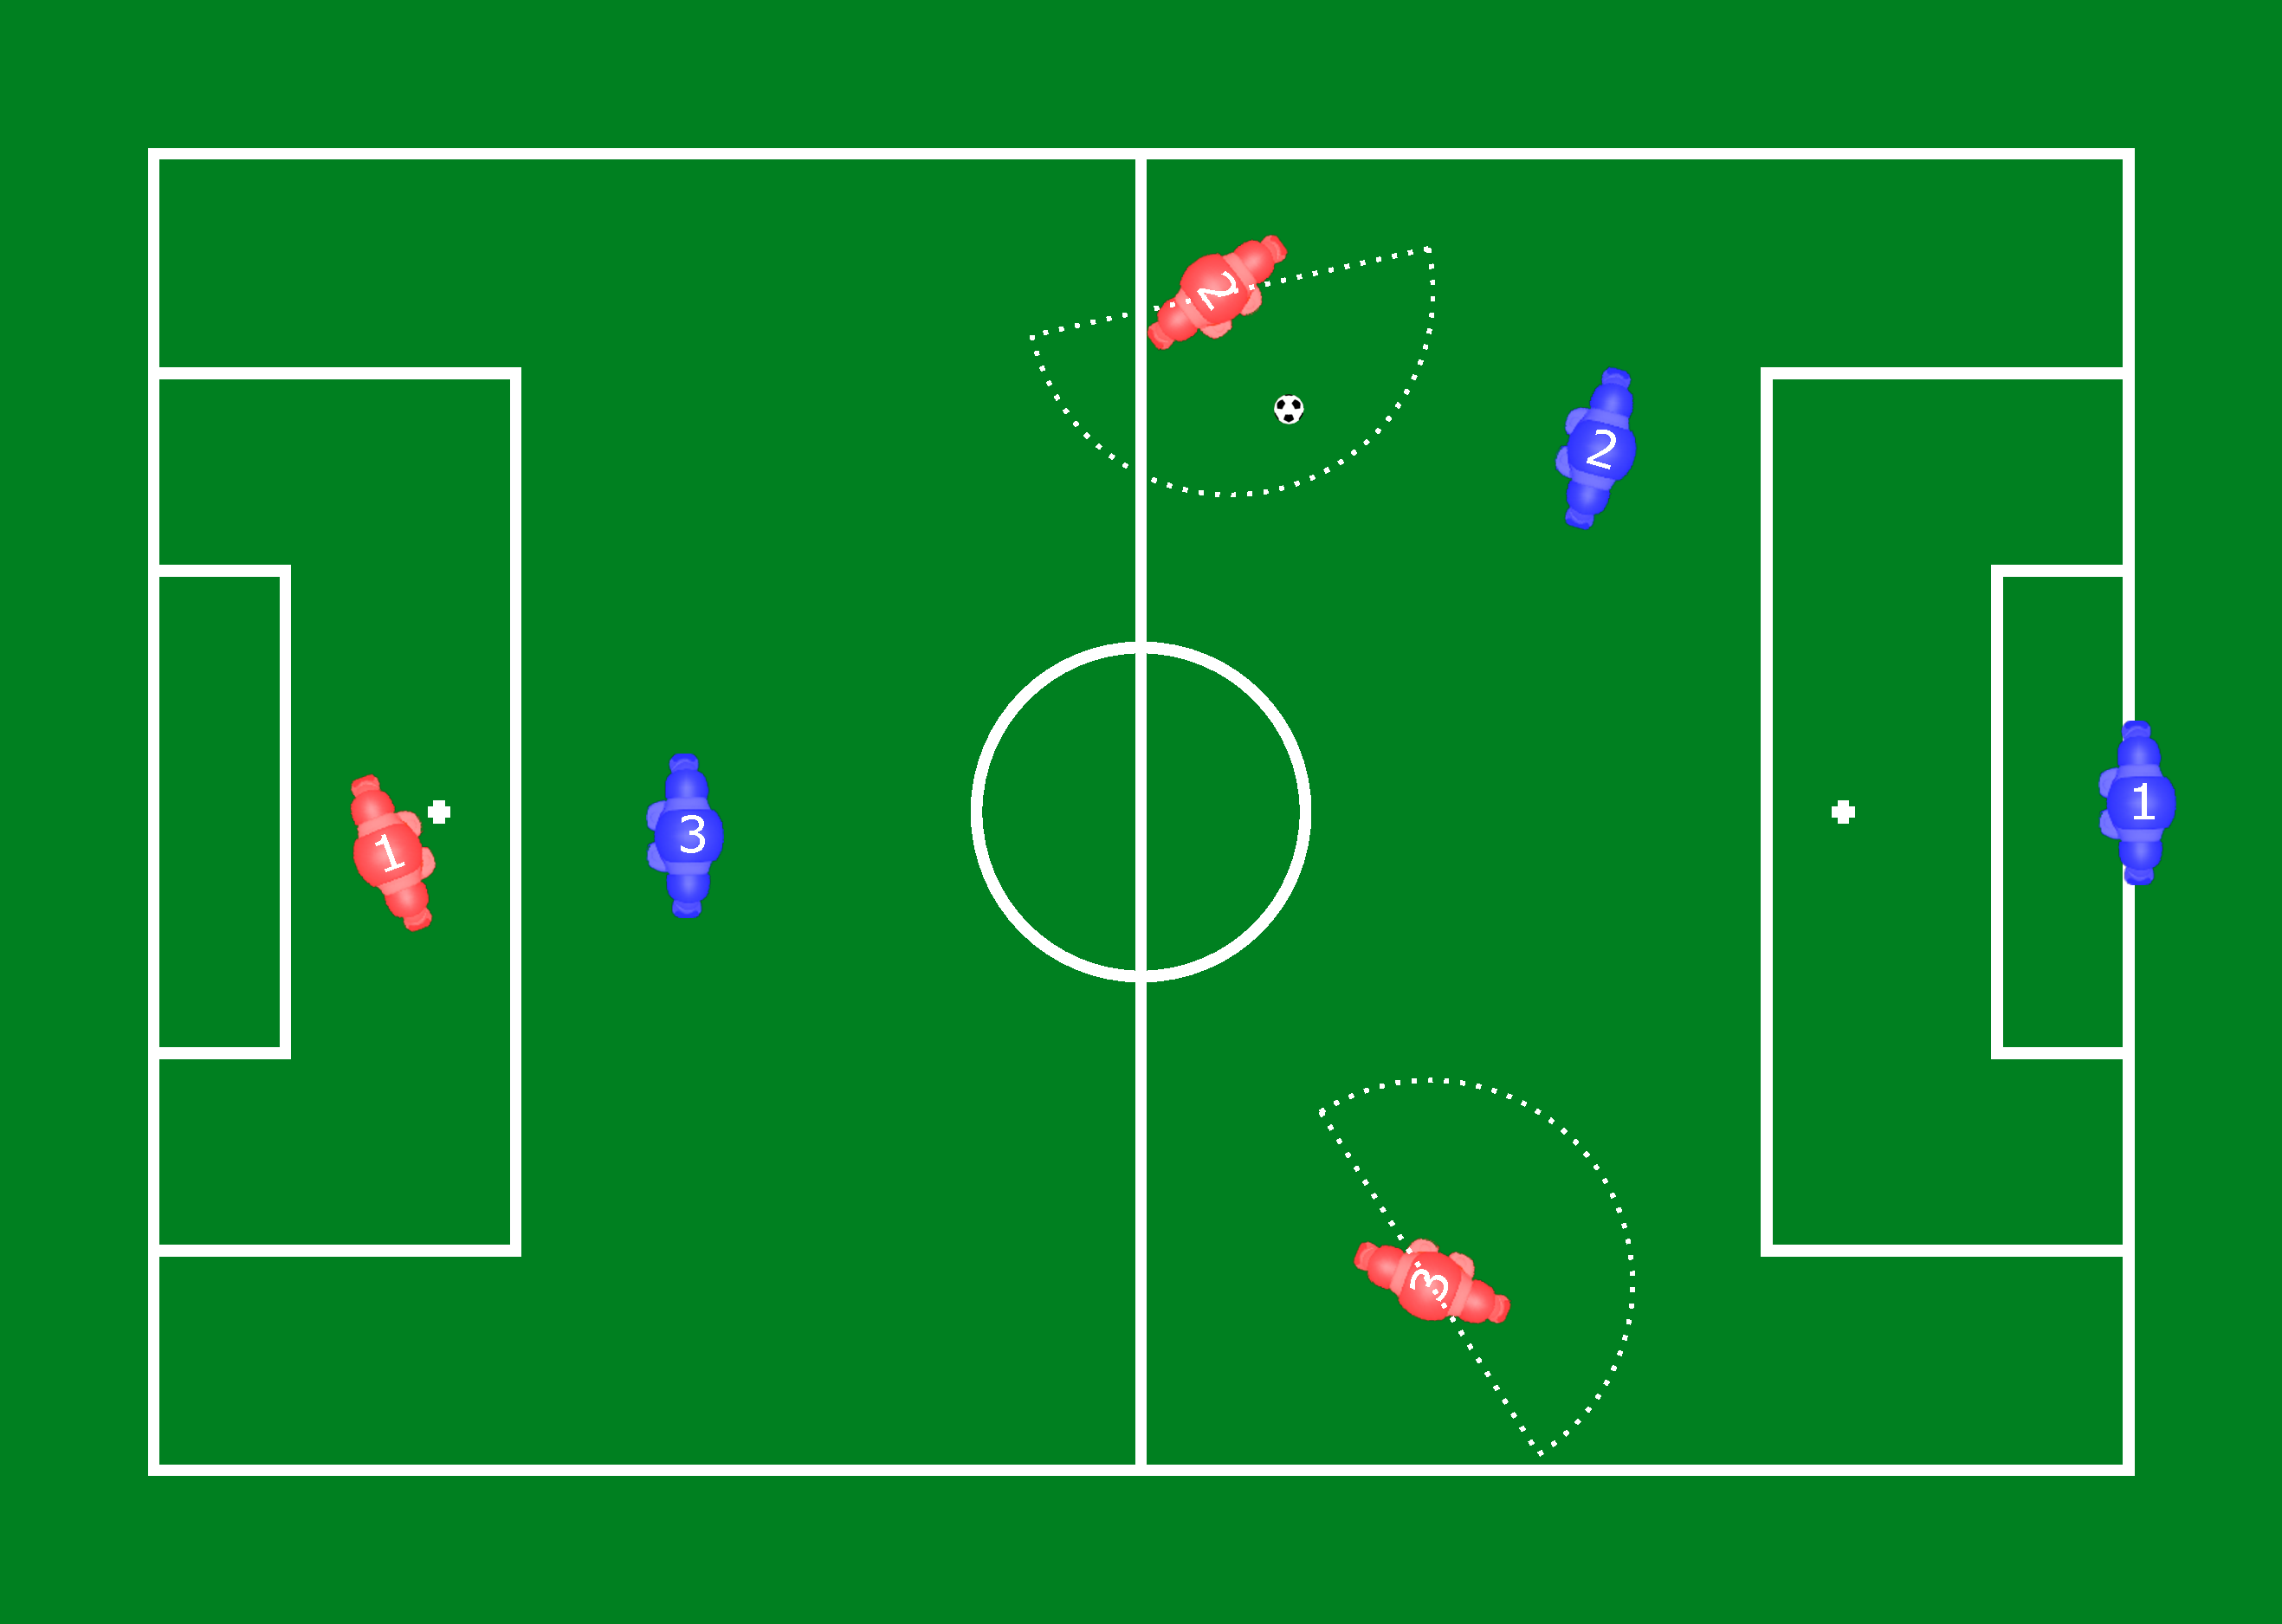
\includegraphics[width=1\columnwidth]{figs/dbhc_arcs.pdf}
		\caption{Possible challenge situation with {\color{red} attacking (red)} robots already oriented towards their targets. The arcs for a valid pass are indicated with dashed line style. Please note the possible difference between robot orientation and valid arcs.}
		\label{fig:ball_handling_arc_positions}
	\end{center}
\end{figure}

\subsection{Challenge Scoring}
\label{sec:Challenge_scoring}
In each run the GameController measures the execution time from initial whistle until the run is stopped by one of the following criteria:

\begin{itemize}
	\item A goal is scored after at least two passes, out of the following list, have been executed:
	\begin{itemize}
		\item valid pass,
		\item semi-valid pass,
		\item substantial pass attempt.
	\end{itemize}
	\item A defender (except the goalkeeper) touches the ball.
	\item Ball leaves the field outside the defending goal area.
	\item An attacker pushes.
	\item There is only one attacker left on the field.
	\item A run exceeds \qty{4}{\minute} execution time.
	\item Attacking team is not communicating with the GameController.
\end{itemize}

In the case that a goal gets scored before two passes (see list above) were executed, or the ball leaves the field within the defending goal area, the ball gets placed on the closest goal kick spot.

The score for the attacking team in a run will be calculated based on the following rules:

\begin{enumerate}
	\item For the first two passes, add 
	\begin{enumerate}
		\item \textbf{valid pass}: \qty{30}{} points.
		\item \textbf{semi-valid pass}: \qty{20}{} points.
		\item \textbf{substantial pass attempt}: \qty{10}{} points.
	\end{enumerate}
	\item For a third pass, add
	\begin{enumerate}
		\item \textbf{valid pass}: \qty{20}{} points.
		\item \textbf{semi-valid pass}: \qty{13}{} points.
		\item \textbf{substantial pass attempt}: \qty{6}{} points.
	\end{enumerate}
	\item For a fourth pass, add
	\begin{enumerate}
		\item \textbf{valid pass}: \qty{10}{} points.
		\item \textbf{semi-valid pass}: \qty{6}{} points.
		\item \textbf{substantial pass attempt}: \qty{3}{} points.
	\end{enumerate}
	\item For a goal after at least two passes, add \qty{50}{} points.
	\item The time measured counts and can lead to \qty{120}{} points if \qty{0}{\second} are needed and \qty{0}{} points if \qty{240}{\second} are needed. In between full points (rounded) will be awarded linearly. \\
	\textit{However these points are not awarded if the run was stopped by a stopping criteria different to scoring a goal, see above.}
	\item If an attacking robot has been pushed by a defender, subtract \qty{20}{\second} of the time measured.
\end{enumerate}

The final score is the sum of the two best runs out of the three runs.

\subsection{Defender image}
\label{sec:Challenge_image}
Common defender images can be provided by the community with a standardized setup procedure and with automatic calibration. Every team can propose such an image until 2023-05-14. The image will be tested until 2023-05-31 if they match the requirements and afterwards published. If not, the team gets feedback and has the opportunity to hand in a revised image. If teams want to test their attackers before this deadline the old images from 2022 and the old GameController can be used.

\begin{enumerate}
	\item One image applying to the standard button interface, using autonomous calibration and receives it player number through a text file on USB-stick.
	\item Existence of documentation on how to flash, how to operate a robot, how to handle issues.
	\item Does it apply to the rules?
	\item Does it operate robustly?
	\item Does it defend according to the rules?
\end{enumerate}


% !TeX root = ../SPL-Challenges.tex
% !TeX spellcheck = en_US
\section{Data Minimization Challenge} % TODO: I hope there is a better name for this challenge


\end{document}
